\documentclass{article}
\usepackage[margin=0.3cm]{geometry}
\usepackage{url}
\usepackage{multicol}
\usepackage{amsmath}
\usepackage{esint}
\usepackage{amsfonts}
\usepackage{tikz}
\usetikzlibrary{decorations.pathmorphing}
\usepackage{amsmath,amssymb}

\usepackage{colortbl}
\usepackage{xcolor}
\usepackage{mathtools}
\usepackage{amsmath,amssymb}
\usepackage{enumitem}

\newcommand{\blank}[1]{\hspace*{#1}\linebreak[0]}

\tikzstyle{mybox} = [draw=black, fill=white, very thick,
    rectangle, rounded corners, inner sep=10pt, inner ysep=10pt]
\tikzstyle{fancytitle} =[fill=black, text=white, font=\bfseries]

\begin{document}
\begin{center}{\huge{\textbf{CS 480 Cheat Sheet}}}
\end{center}

\begin{center}
\begin{multicols*}{2}
%------------ Perceptron ---------------------
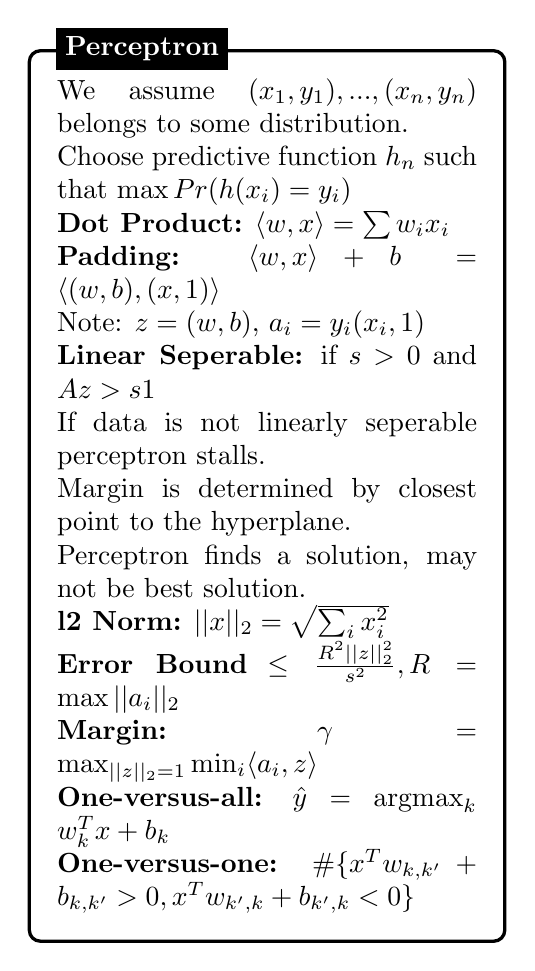
\begin{tikzpicture}
\node [mybox] (box){%
    \begin{minipage}{0.44\textwidth}
    We assume $(x_1,y_1),...,(x_n,y_n)$ belongs to some distribution.\\
    Choose predictive function  $h_n$ such that $\max Pr(h(x_i) = y_i)$ \\
    \textbf{Dot Product:} $ \langle w, x  \rangle = \sum w_ix_i $\\
    \textbf{Padding:} $\langle w, x  \rangle + b = \langle (w, b), (x, 1) \rangle$ \\
    Note: $z = (w,b)$, $a_i = y_i(x_i,1)$\\
    \textbf{Linear Seperable:} if $s>0$ and $Az > s1$ \\
If data is not linearly seperable perceptron stalls. \\
Margin is determined by closest point to the hyperplane. \\
Perceptron finds a solution, may not be best solution. \\
    \textbf{l2 Norm:} $||x||_2 = \sqrt{\sum_ix_i^2}$ \\
    \textbf{Error Bound} $\leq \frac{R^2||z||^2_2}{s^2}, R = \max||a_i||_2$  \\
    \textbf{Margin:} $\gamma = \max_{||z||_2 = 1} \min_i \langle a_i, z \rangle$ \\
    \textbf{One-versus-all:}  $\hat{y} = \text{argmax}_k$ $w_k^Tx + b_k $ \\
    \textbf{One-versus-one:} $\# \{ x^Tw_{k,k'} + b_{k,k'} > 0, x^Tw_{k',k} + b_{k',k} < 0 \}$
    \end{minipage}
};
\node[fancytitle, right=10pt] at (box.north west) {Perceptron};
\end{tikzpicture}

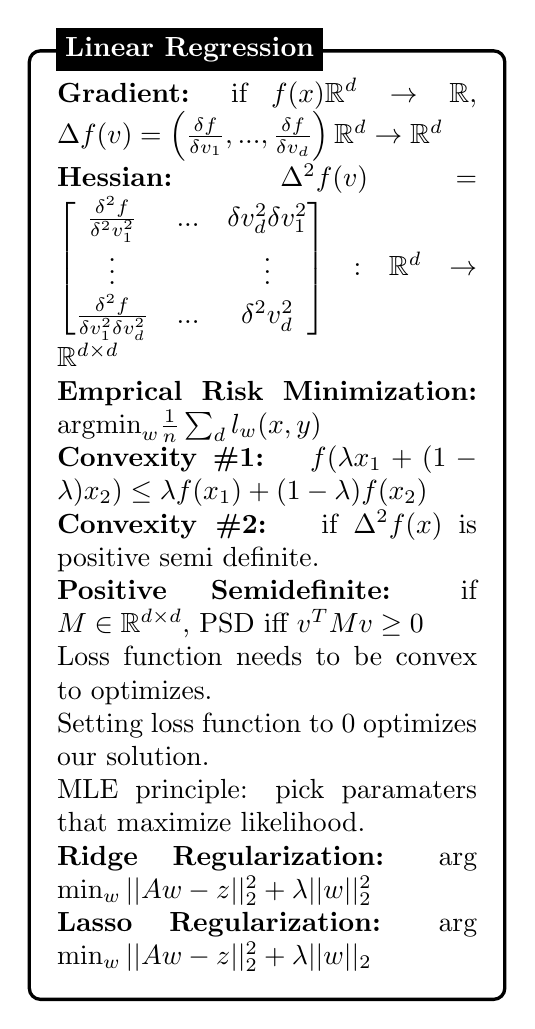
\begin{tikzpicture}
\node [mybox] (box){%
    \begin{minipage}{0.44\textwidth}
	\textbf{Gradient:} if $f(x) \mathbb{R}^d \rightarrow \mathbb{R}$, $\Delta f(v) = \left( \frac{\delta f}{\delta v_1}, ..., \frac{\delta f}{\delta v_d}  \right) \mathbb{R}^d \rightarrow \mathbb{R}^d$ \\
	\textbf{Hessian:} $\Delta^2 f(v) = \begin{bmatrix}
\frac{\delta^2f}{\delta^2 v_1^2} & ... & \delta v_d^2\delta v_1^2 \\
\vdots &  & \vdots \\
\frac{\delta^2f}{\delta v_1^2\delta v_d^2} & ... & \delta^2 v_d^2
\end{bmatrix}: \mathbb{R}^d \rightarrow\mathbb{R}^{d\times d} $\\
\textbf{Emprical Risk Minimization:} $\text{argmin}_w \frac{1}{n}\sum_d l_w(x,y)$ \\
\textbf{Convexity \#1: } $f(\lambda x_1 + (1- \lambda)x_2) \leq \lambda f(x_1) + (1-\lambda)f(x_2)$ \\
\textbf{Convexity \#2: } if $\Delta^2f(x)$ is positive semi definite. \\
\textbf{Positive Semidefinite:} if $M \in \mathbb{R}^{d \times d}$, PSD iff $v^TMv \geq 0$\\
Loss function needs to be convex to optimizes.\\
Setting loss function to 0 optimizes our solution.\\
MLE principle: pick paramaters that maximize likelihood.\\
\textbf{Ridge Regularization:} arg $\min_w ||Aw-z||^2_2 + \lambda||w||^2_2
$\\
\textbf{Lasso Regularization:} arg $\min_w ||Aw-z||^2_2 + \lambda||w||_2
$    \end{minipage}
};
\node[fancytitle, right=10pt] at (box.north west) {Linear Regression};
\end{tikzpicture}

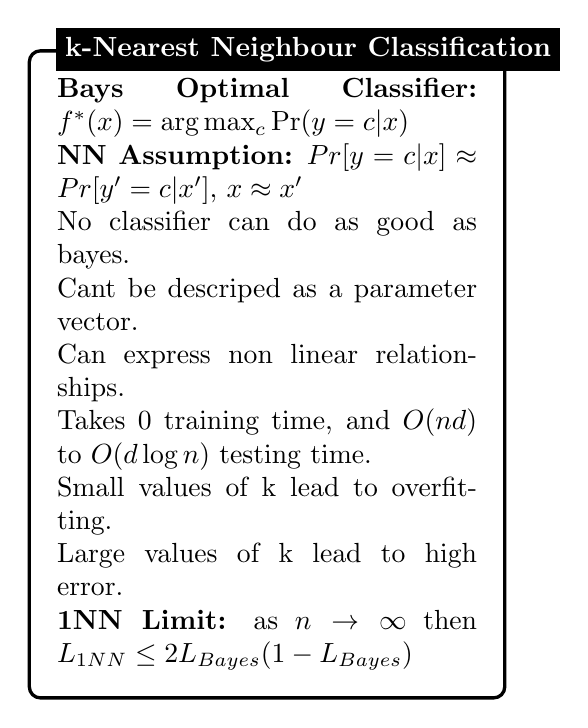
\begin{tikzpicture}
\node [mybox] (box){%
    \begin{minipage}{0.44\textwidth}
	\textbf{Bays Optimal Classifier:} $f^*(x) = \text{arg}\max_c\text{Pr}(y=c|x)$\\
	\textbf{NN Assumption:} $Pr[y=c|x] \approx Pr[y'=c|x']$, $x\approx x'$\\
	No classifier can do as good as bayes.\\
	Cant be descriped as a parameter vector.\\
	Can express non linear relationships.\\
	Takes 0 training time, and $O(nd)$  to $O(d\log n)$ testing time.\\
	Small values of k lead to overfitting. \\
	Large values of k lead to high error. \\
	\textbf{1NN Limit:} as $n \rightarrow \infty$ then $L_{1NN} \leq 2L_{Bayes}(1 - L_{Bayes})$

    \end{minipage}
};
\node[fancytitle, right=10pt] at (box.north west) {k-Nearest Neighbour Classification};
\end{tikzpicture}

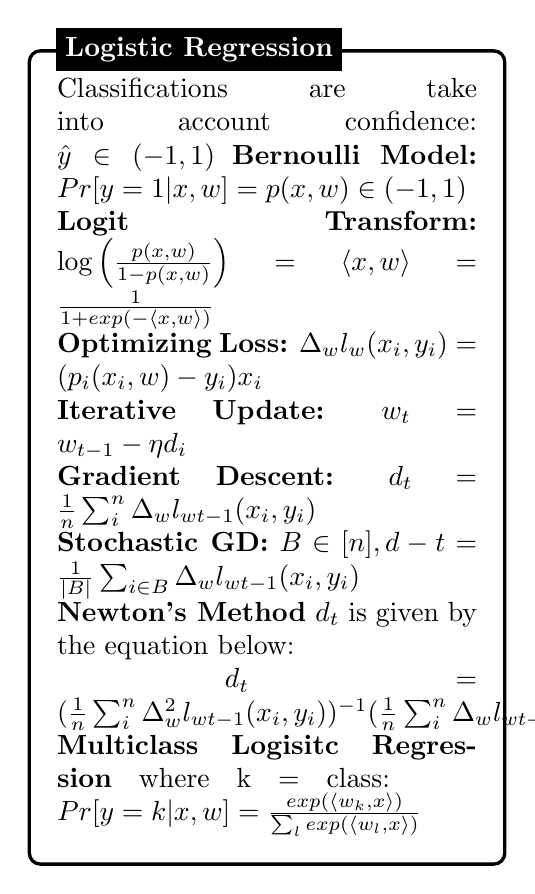
\begin{tikzpicture}
\node [mybox] (box){%
    \begin{minipage}{0.44\textwidth}
		Classifications are take into account confidence: $\hat{y} \in (-1,1)$
		\textbf{Bernoulli Model:} $Pr[y=1|x,w] = p(x,w) \in (-1,1) $ \\
		\textbf{Logit Transform:} $\log\left( \frac{p(x,w)}{1-p(x,w)}\right) = \langle x,w\rangle = \frac{1}{1+exp(-\langle x,w\rangle)}$\\
		\textbf{Optimizing Loss:} $\Delta_w l_w(x_i,y_i) = (p_i(x_i,w)-y_i)x_i$\\
		\textbf{Iterative Update:} $w_t = w_{t-1}-\eta d_i$ \\
		\textbf{Gradient Descent:} $d_t = \frac{1}{n}\sum_i^n\Delta_w l_{wt-1}(x_i,y_i)$ \\
		\textbf{Stochastic GD:} $B \in [n], d-t = \frac{1}{|B|}\sum_{i\in B}\Delta_w l_{wt-1}(x_i,y_i)$ \\
		\textbf{Newton's Method} $d_t$ is given by the equation below:\\
		\blank{0.5cm} $d_t = (\frac{1}{n}\sum_i^n\Delta^2_w l_{wt-1}(x_i,y_i))^{-1}(\frac{1}{n}\sum_i^n\Delta_w l_{wt-1}(x_i,y_i))$\\
		\textbf{Multiclass Logisitc Regression} where k = class:
		\blank{0.5cm} $Pr[y=k|x,w] = \frac{exp(\langle w_k,x \rangle)}{\sum_l exp(\langle w_l,x \rangle)} $
    \end{minipage}
};
\node[fancytitle, right=10pt] at (box.north west) {Logistic Regression};
\end{tikzpicture}

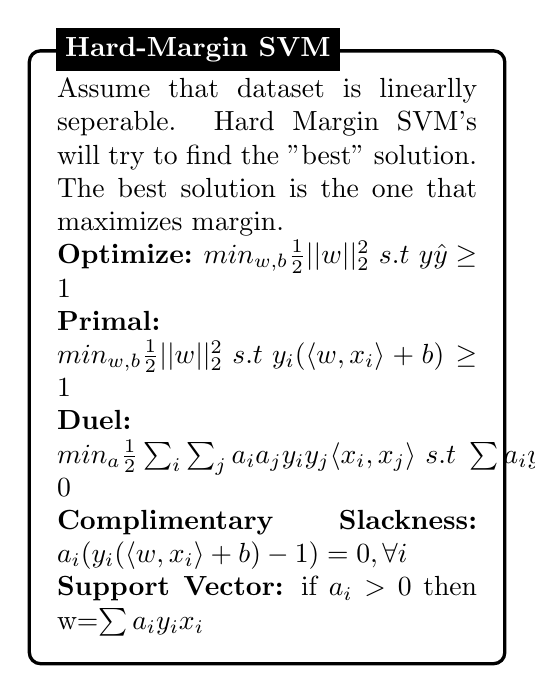
\begin{tikzpicture}
\node [mybox] (box){%
    \begin{minipage}{0.44\textwidth}
		Assume that dataset is linearlly seperable. Hard Margin SVM's will try to find the "best" solution. The best solution is the one that maximizes margin. \\
		\textbf{Optimize:} $min_{w,b}\frac{1}{2}||w||_2^2 \text{ } s.t \text{ } y\hat{y}\geq 1$ \\
		\textbf{Primal:} $min_{w,b}\frac{1}{2}||w||_2^2 \text{ } s.t \text{ } y_i(\langle w, x_i \rangle + b )\geq 1$ \\
		\textbf{Duel:} $min_{a}\frac{1}{2}\sum_i\sum_j a_ia_jy_iy_j \langle x_i, x_j \rangle \text{ } s.t \text{ } \sum a_iy_i = 0$ \\
		\textbf{Complimentary Slackness:} $a_i(y_i(\langle w, x_i \rangle +b) -1) = 0, \forall i$\\
		\textbf{Support Vector:} if $a_i > 0$ then w=$\sum a_iy_ix_i$
    \end{minipage}
};
\node[fancytitle, right=10pt] at (box.north west) {Hard-Margin SVM};
\end{tikzpicture}

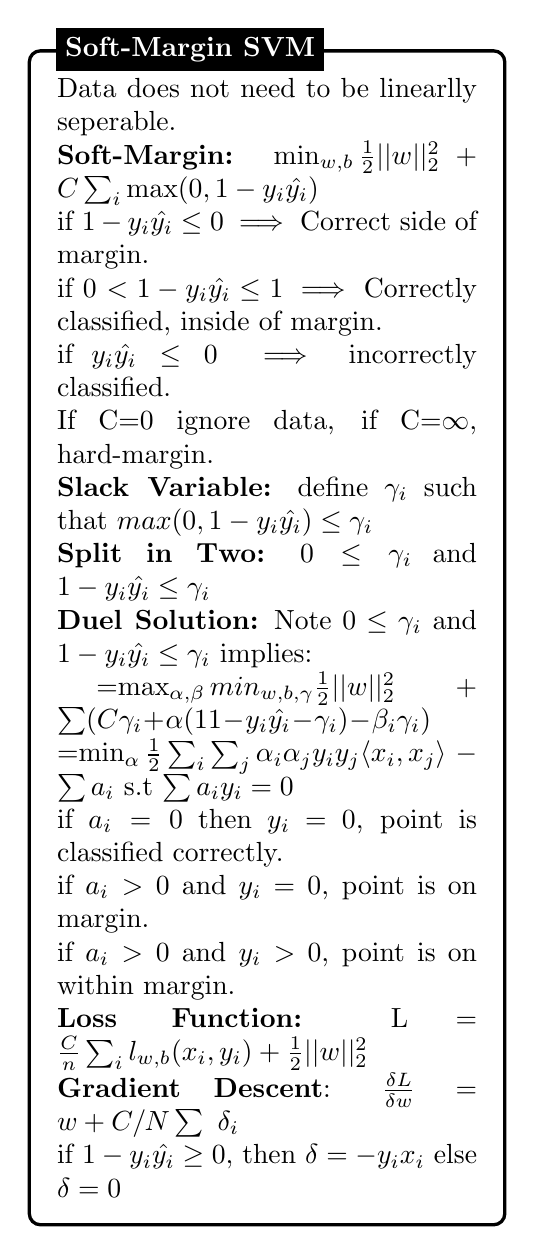
\begin{tikzpicture}
\node [mybox] (box){%
    \begin{minipage}{0.44\textwidth}
		Data does not need to be linearlly seperable.\\
	\textbf{Soft-Margin:} $\min_{w,b} \frac{1}{2}||w||_2^2 + C \sum_i \max(0, 1-y_i\hat{y_i})$\\
	if $1-y_i\hat{y_i} \leq 0 \implies$ Correct side of margin.\\
	if 0 $< 1-y_i\hat{y_i} \leq 1 \implies$ Correctly classified, inside  of margin. \\
	if $y_i\hat{y_i} \leq 0 \implies$ incorrectly classified. \\
	If C=0 ignore data, if C=$\infty$, hard-margin. \\
	\textbf{Slack Variable:} define $\gamma_i$ such that $max(0,1-y_i\hat{y_i}) \leq \gamma_i$\\
	\textbf{Split in Two:} $0 \leq \gamma_i$ and $1-y_i\hat{y_i} \leq \gamma_i$ \\
	\textbf{Duel Solution:} Note $0 \leq \gamma_i$ and $1-y_i\hat{y_i} \leq \gamma_i$ implies:\\
	\blank{0.5cm}=$ \max_{\alpha, \beta} min_{w,b,\gamma} \frac{1}{2} ||w||^2_2+\sum(C\gamma_i + \alpha(11-y_i\hat{y_i} - \gamma_i) - \beta_i\gamma_i)$
	\blank{0.5cm}=$\min_\alpha \frac{1}{2}\sum_i\sum_j\alpha_i\alpha_jy_iy_j\langle x_i, x_j \rangle - \sum a_i$ s.t $\sum a_iy_i = 0$\\
	if $a_i=0$ then $y_i$ = 0, point is classified correctly. \\
	if $a_i>0$ and $y_i$ = 0, point is on margin. \\
	if $a_i>0$ and $y_i >$  0, point is on within margin.\\
	\textbf{Loss Function:} L = $ \frac{C}{n}\sum_i l_{w,b}(x_i,y_i) + \frac{1}{2}||w||^2_2$\\
	\textbf{Gradient Descent}: $\frac{\delta L}{\delta w} = w + C/N\sum\ \delta_i$ \\
	if $1-y_i\hat{y_i}\geq 0,$ then $\delta = -y_ix_i $ else $\delta = 0$
    \end{minipage}
};
\node[fancytitle, right=10pt] at (box.north west) {Soft-Margin SVM};
\end{tikzpicture}

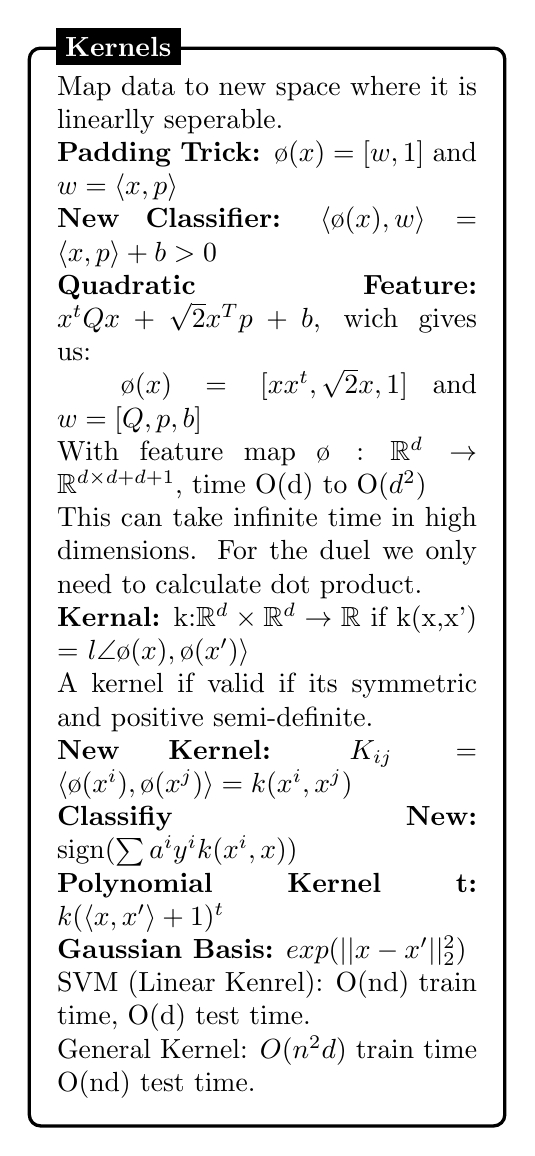
\begin{tikzpicture}
\node [mybox] (box){%
    \begin{minipage}{0.44\textwidth}
	Map data to new space where it is linearlly seperable.\\
	\textbf{Padding Trick: }$\o(x) = [w,1]$ and $w = \langle x,p \rangle$\\
	\textbf{New Classifier:} $\langle \o(x),w \rangle = \langle x,p \rangle +b > 0$\\
	\textbf{Quadratic Feature:} $x^tQx + \sqrt{2}x^Tp + b$, wich gives us:\\
	\blank{0.5cm} $\o(x) = [xx^t,\sqrt{2}x,1]$ and $w= [Q,p,b]$\\
	With feature map $\o:\mathbb{R}^d \rightarrow \mathbb{R}^{d\times d +d + 1}$, time O(d) to O($d^2$)\\
	This can take infinite time in high dimensions.
	For the duel we only need to calculate dot product.\\
	\textbf{Kernal:} k:$\mathbb{R}^d\times\mathbb{R}^d\rightarrow \mathbb{R}$ if k(x,x') = $\l \angle \o(x), \o(x') \rangle$\\
	A kernel if valid if its symmetric and positive semi-definite.\\
	\textbf{New Kernel:} $K_{ij} = \langle \o(x^i), \o(x^j) \rangle = k(x^i, x^j)$\\
	\textbf{Classifiy New:} sign($\sum a^iy^ik(x^i,x))$ \\
	\textbf{Polynomial Kernel t:} $k(\langle x,x' \rangle + 1)^t$\\
	\textbf{Gaussian Basis:} $exp(||x-x'||^2_2)$\\
	SVM (Linear Kenrel): O(nd) train time, O(d) test time.\\
	General Kernel: $O(n^2d)$ train time O(nd) test time.
    \end{minipage}
};
\node[fancytitle, right=10pt] at (box.north west) {Kernels};
\end{tikzpicture}

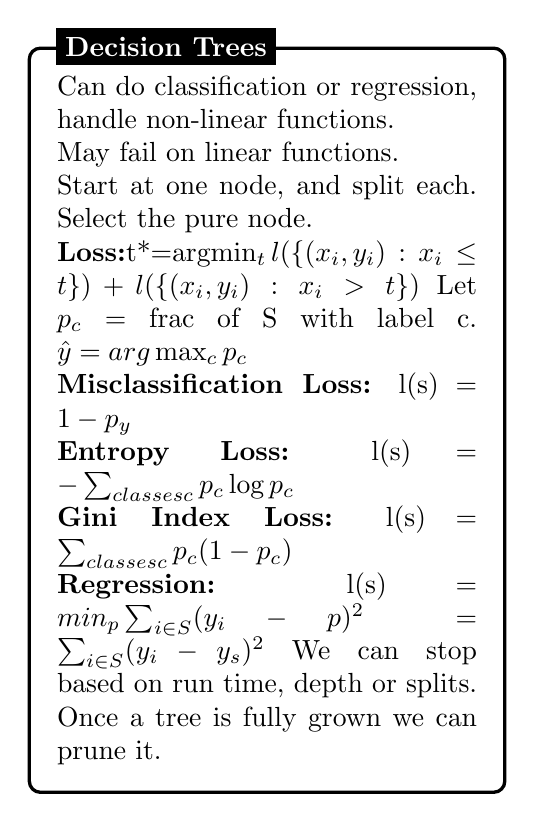
\begin{tikzpicture}
\node [mybox] (box){%
    \begin{minipage}{0.44\textwidth}
	Can do classification or regression, handle non-linear functions.\\
	May fail on linear functions.\\
	Start at one node, and split each. Select the pure node.\\
	\textbf{Loss:}t*=arg$\min_t l(\{(x_i,y_i):x_i \leq t \}) + l(\{(x_i,y_i):x_i > t \})$
	Let $p_c$ = frac of S with label c. $\hat{y} = arg \max_c p_c$\\
	\textbf{Misclassification Loss:} l(s) = $1-p_y$\\
	\textbf{Entropy Loss:} l(s) = $-\sum_{classes c} p_c \log p_c$\\
	\textbf{Gini Index Loss:} l(s) = $\sum_{classes c} p_c (1-p_c)$ \\
	\textbf{Regression:} l(s) = $min_p \sum_{i \in S}(y_i -p)^2 = \sum_{i \in S}(y_i -y_s)^2$
	We can stop based on run time, depth or splits. \\
	Once a tree is fully grown we can prune it. 
    \end{minipage}
};
\node[fancytitle, right=10pt] at (box.north west) {Decision Trees};
\end{tikzpicture}

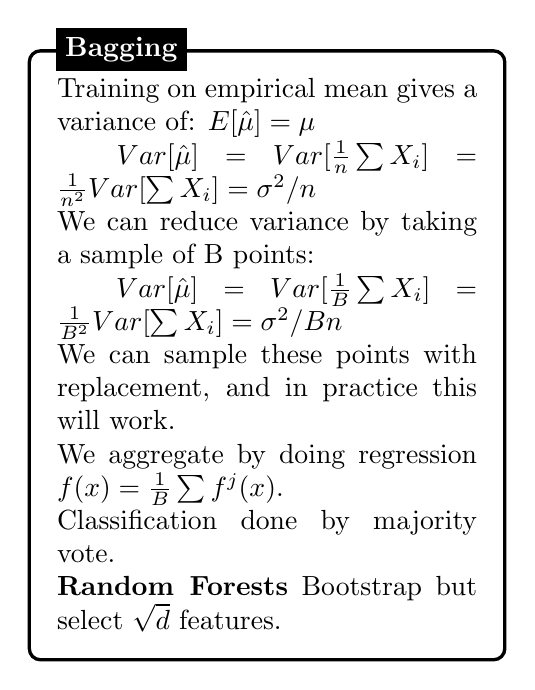
\begin{tikzpicture}
\node [mybox] (box){%
    \begin{minipage}{0.44\textwidth}
	Training on empirical mean gives a variance of: $E[\hat{\mu}] = \mu$\\
	\blank{0.5cm} $Var[\hat{\mu}] = Var [\frac{1}{n}\sum X_i] = \frac{1}{n^2}Var[\sum X_i] = \sigma^2/n$\\
	We can reduce variance by taking a sample of B points:\\
	\blank{0.5cm} $Var[\hat{\mu}] = Var [\frac{1}{B}\sum X_i] = \frac{1}{B^2}Var[\sum X_i] = \sigma^2/Bn$\\
	We can sample these points with replacement, and in practice this will work. \\
	We aggregate by doing regression $f(x) = \frac{1}{B}\sum f^j(x)$. \\
	Classification done by majority vote.\\
	\textbf{Random Forests} Bootstrap but select $\sqrt d$ features.
    \end{minipage}
};
\node[fancytitle, right=10pt] at (box.north west) {Bagging};
\end{tikzpicture}

\begin{tikzpicture}
\node [mybox] (box){%
    \begin{minipage}{0.44\textwidth}
	Neural Networks learn mapping from the data.\\
	\textbf{Sigmoid:} $\sigma(t) = \frac{1}{1+e^{-t}}$\\
	$\hat{y} = \frac{1}{1+exp(-\langle w,x \rangle -b} )$\\
	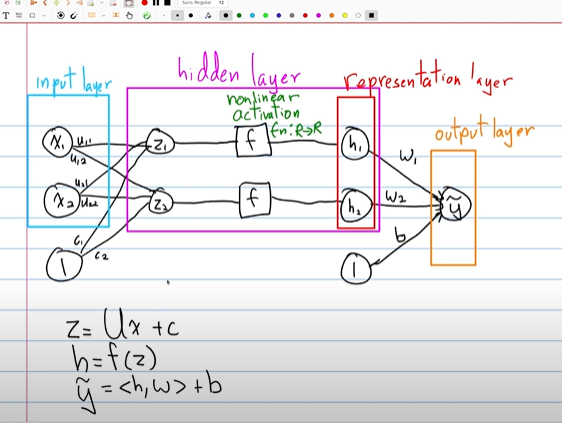
\includegraphics[scale=0.8
	]{mlp.png}\\
	\textbf{ReLU(t)} = $\max(0,t)$\\ 
	\textbf{Loss} $l_\theta(x,y) = -\sum^my_ilogy_i$\\
	\textbf{Tanh(t)}= $\frac{e^t-e^{-1}}{e^t+e^{-t}}$\\
	\textbf{Gradient Descent} $\theta^t=\theta^{t-1} - \eta \Delta L_{\theta{t-1}}$\\
	\textbf{Chain rule:} $\frac{dz}{dx} = \frac{dz}{dy}\frac{dy}{dx}$\\
	Any contionus function can be approximated well by a 2 layer nn.
    \end{minipage}
};
\node[fancytitle, right=10pt] at (box.north west) {Multilayer Perceptron};
\end{tikzpicture}

\begin{tikzpicture}
\node [mybox] (box){%
    \begin{minipage}{0.44\textwidth}
	Most neural networks have many paramaters. We can minimize overfiting with:\\
	\blank{0.5cm} Regularazation loss, gradient descent, and equivalently:\\
	\blank{0.5cm} $\theta_t \leftarrow (1-\eta\lambda)\theta_{t-1} - \eta\Delta L{\theta{t-1}})(x,y)$\\
	We can drop nodes and use normlizaiton of features:\\
	mean$ = \frac{1}{n}\sum X_i$, $X_i \leftarrow X_i - \mu$, $\sigma_j^2=\frac{1}{n}\sum X_{i,j}, X_{i,j} = X_{i,j}/\sigma_j$\\
	We do normilizaiton on each batch, such that:\\
	$z^i = W^ih^{i-1} +b^i$ or $h^i = f(z^i)$\\
	We can do normlization on each neuron (batchnorm) or each layer. \\
	\textbf{Batch GD:} $\theta \leftarrow \theta - \eta * \frac{1}{n} \sum \delta l_\theta(x_i, j_i)$, optomize gradient.
	\textbf{Momentum:} $v_t= \gamma v_{t-1} + (1-\gamma)\mu, \theta_t \leftarrow \theta_{t-1} - v_t$ 
	\textbf{RMSProp} let $g\in R^p$, $G_{t,i} = \sum^tg^2_{j,i}\text{and } \theta_t \leftarrow \theta_{t-1}-\frac{\mu}{\sqrt{G_{t,i}+\epsilon}}g_{t,i}$\\
	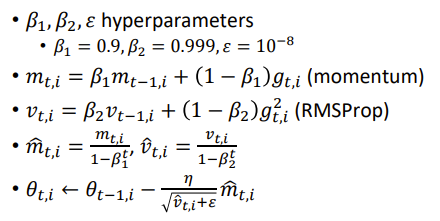
\includegraphics[scale=0.6]{2.png}
    \end{minipage}
};
\node[fancytitle, right=10pt] at (box.north west) {Deep Networks};
\end{tikzpicture}

\begin{tikzpicture}
\node [mybox] (box){%
    \begin{minipage}{0.44\textwidth}
	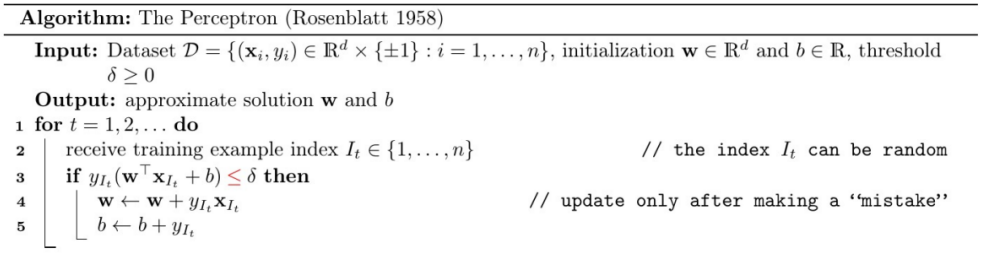
\includegraphics[width=9cm, height=3cm]{3.png}
    \end{minipage}
};
\node[fancytitle, right=10pt] at (box.north west) {[Perceptron] Algorthim};
\end{tikzpicture}

\begin{tikzpicture}
\node [mybox] (box){%
    \begin{minipage}{0.44\textwidth}
	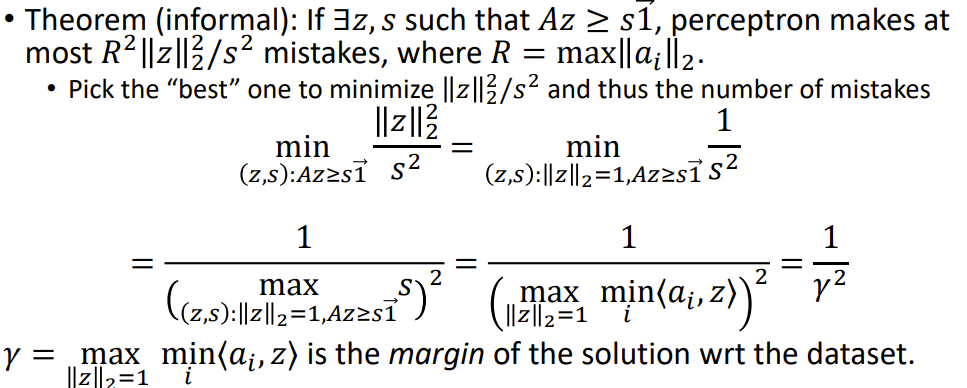
\includegraphics[width=9cm, height=2.5cm]{4.png}
    \end{minipage}
};
\node[fancytitle, right=10pt] at (box.north west) {[Perceptron] Error Bound};

\end{tikzpicture}

\begin{tikzpicture}
\node [mybox] (box){%
    \begin{minipage}{0.44\textwidth}
	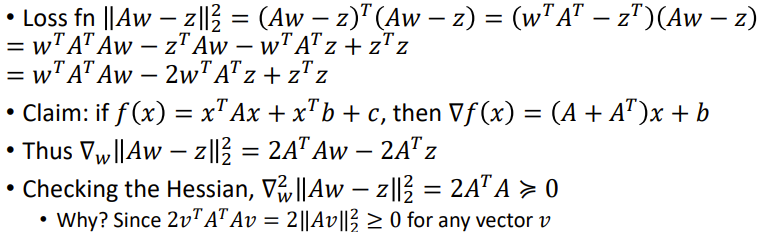
\includegraphics[width=9cm, height=2.5cm]{5.png}
    \end{minipage}
};
\node[fancytitle, right=10pt] at (box.north west) {[Linear Regression] Convexity of Loss Function};
\end{tikzpicture}

\begin{tikzpicture}
\node [mybox] (box){%
    \begin{minipage}{0.44\textwidth}
	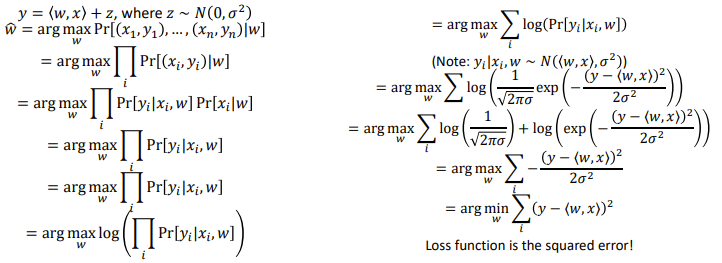
\includegraphics[width=9cm, height=4cm]{6.png}
    \end{minipage}
};
\node[fancytitle, right=10pt] at (box.north west) {[Linear Regression] Deriving MLE};
\end{tikzpicture}

\begin{tikzpicture}
\node [mybox] (box){%
    \begin{minipage}{0.44\textwidth}
	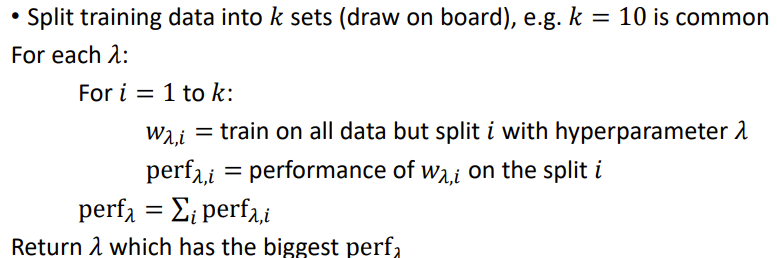
\includegraphics[width=9cm, height=2.5cm]{7.png}
    \end{minipage}
};
\node[fancytitle, right=10pt] at (box.north west) {[Linear Regression] Cross Validation};
\end{tikzpicture}

\begin{tikzpicture}
\node [mybox] (box){%
    \begin{minipage}{0.44\textwidth}
	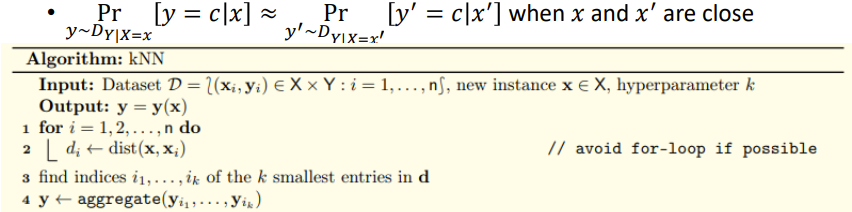
\includegraphics[width=9cm, height=2.5cm]{8.png}
    \end{minipage}
};
\node[fancytitle, right=10pt] at (box.north west) {[KNN] Algorthim};
\end{tikzpicture}

\begin{tikzpicture}
\node [mybox] (box){%
    \begin{minipage}{0.44\textwidth}
	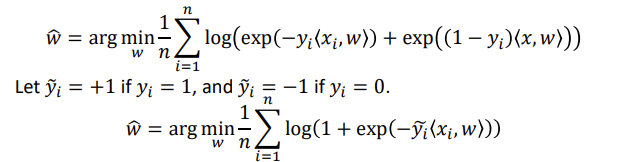
\includegraphics[width=9cm, height=2.5cm]{10.png}
    \end{minipage}
};
\node[fancytitle, right=10pt] at (box.north west) {[Logistic Regression] MLE of $\hat{w}$};
\end{tikzpicture}

\begin{tikzpicture}
\node [mybox] (box){%
    \begin{minipage}{0.44\textwidth}
	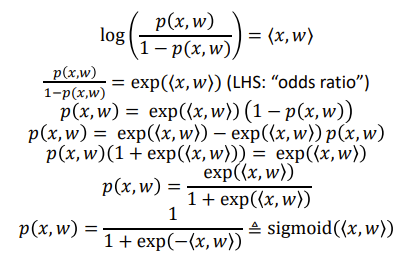
\includegraphics[width=9cm, height=4cm]{9.png}
    \end{minipage}
};
\node[fancytitle, right=10pt] at (box.north west) {[Logistic Regression] Logit Transform};
\end{tikzpicture}

\begin{tikzpicture}
\node [mybox] (box){%
    \begin{minipage}{0.44\textwidth}
	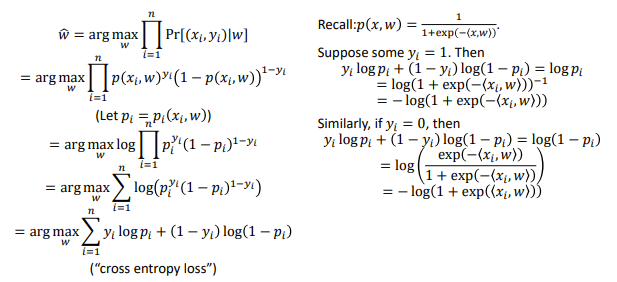
\includegraphics[width=9cm, height=5cm]{11.png}
    \end{minipage}
};
\node[fancytitle, right=10pt] at (box.north west) {[Logistic Regression] Deriving MLE \#1};
\end{tikzpicture}

\begin{tikzpicture}
\node [mybox] (box){%
    \begin{minipage}{0.44\textwidth}
	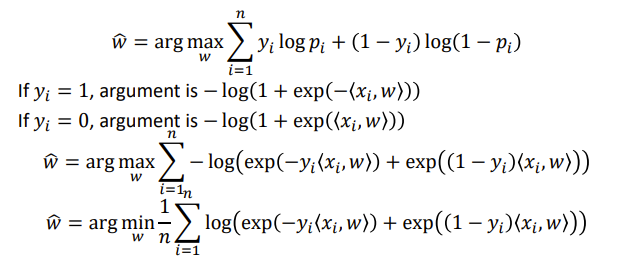
\includegraphics[width=9cm, height=4cm]{12.png}
    \end{minipage}
};
\node[fancytitle, right=10pt] at (box.north west) {[Logistic Regression] Deriving MLE \#2};
\end{tikzpicture}

\begin{tikzpicture}
\node [mybox] (box){%
    \begin{minipage}{0.44\textwidth}
	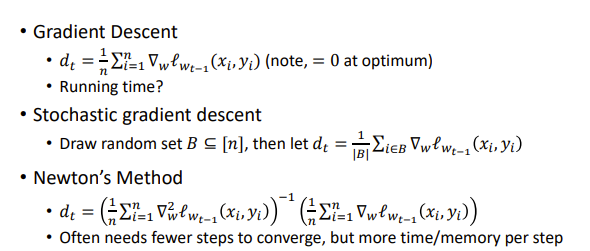
\includegraphics[width=9cm, height=4cm]{13.png}
    \end{minipage}
};
\node[fancytitle, right=10pt] at (box.north west) {[Logistic Regression] $d_t$ Selection};
\end{tikzpicture}

\begin{tikzpicture}
\node [mybox] (box){%
    \begin{minipage}{0.44\textwidth}
	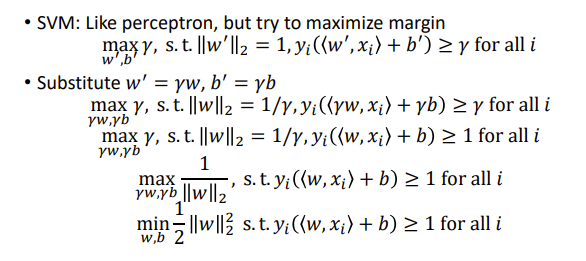
\includegraphics[width=9cm, height=5cm]{14.png}
    \end{minipage}
};
\node[fancytitle, right=10pt] at (box.north west) {[Hard Margin SVM] Goal};
\end{tikzpicture}

\begin{tikzpicture}
\node [mybox] (box){%
    \begin{minipage}{0.44\textwidth}
	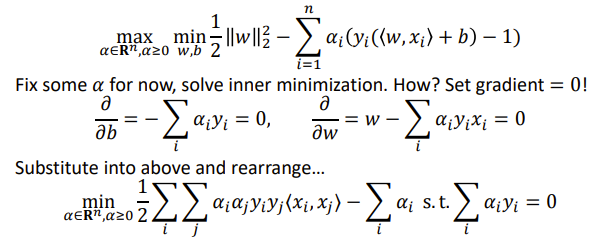
\includegraphics[width=9cm, height=4cm]{15.png}
    \end{minipage}
};
\node[fancytitle, right=10pt] at (box.north west) {[Hard Margin SVM] Duel Formation};
\end{tikzpicture}

\begin{tikzpicture}
\node [mybox] (box){%
    \begin{minipage}{0.44\textwidth}
	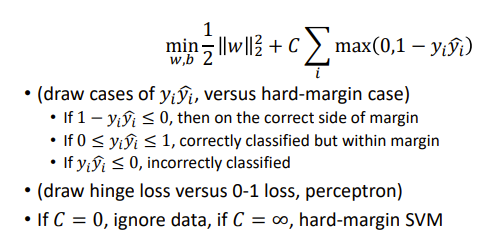
\includegraphics[width=9cm, height=5cm]{16.png}
    \end{minipage}
};
\node[fancytitle, right=10pt] at (box.north west) {[Soft Margin SVM] Goal};
\end{tikzpicture}

\begin{tikzpicture}
\node [mybox] (box){%
    \begin{minipage}{0.44\textwidth}
	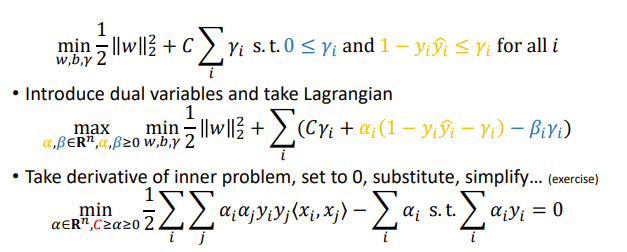
\includegraphics[width=9cm, height=4cm]{17.png}
    \end{minipage}
};
\node[fancytitle, right=10pt] at (box.north west) {[Soft Margin SVM] Duel Formation};
\end{tikzpicture}

\begin{tikzpicture}
\node [mybox] (box){%
    \begin{minipage}{0.44\textwidth}
	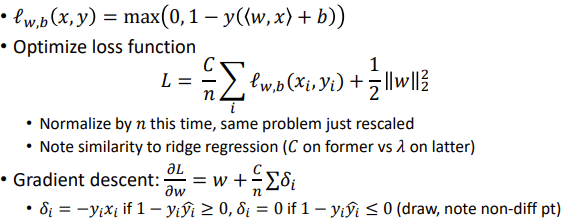
\includegraphics[width=9cm, height=4cm]{18.png}
    \end{minipage}
};
\node[fancytitle, right=10pt] at (box.north west) {[Soft Margin SVM] Optimization};
\end{tikzpicture}

\begin{tikzpicture}
\node [mybox] (box){%
    \begin{minipage}{0.44\textwidth}
	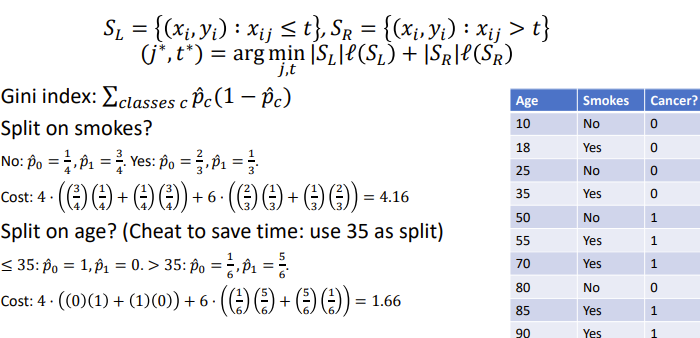
\includegraphics[width=9cm, height=5cm]{19.png}
    \end{minipage}
};
\node[fancytitle, right=10pt] at (box.north west) {[Decision Tree] Example};
\end{tikzpicture}


\begin{tikzpicture}
\node [mybox] (box){%
    \begin{minipage}{0.44\textwidth}
	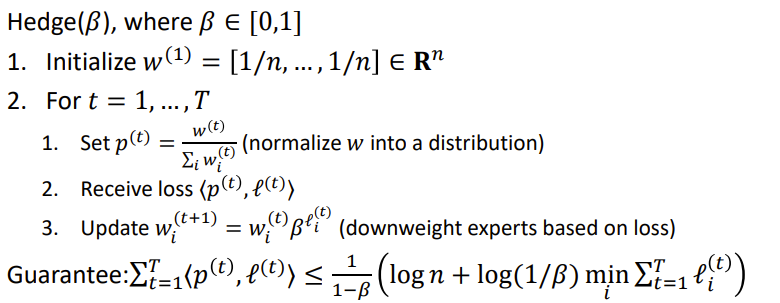
\includegraphics[width=9cm, height=3cm]{20.png}
    \end{minipage}
};
\node[fancytitle, right=10pt] at (box.north west) {[Boosting] Hedge Algorithm};
\end{tikzpicture}

\begin{tikzpicture}
\node [mybox] (box){%
    \begin{minipage}{0.44\textwidth}
	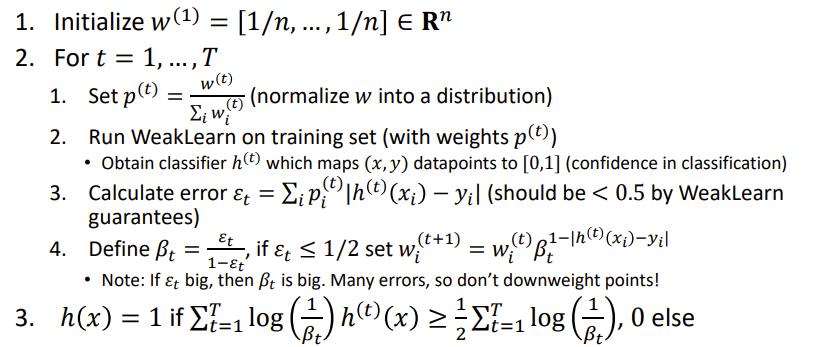
\includegraphics[width=9cm, height=4cm]{21.png}
    \end{minipage}
};
\node[fancytitle, right=10pt] at (box.north west) {[Boosting] AdaBoost Algorithm};
\end{tikzpicture}

\begin{tikzpicture}
\node [mybox] (box){%
    \begin{minipage}{0.44\textwidth}
	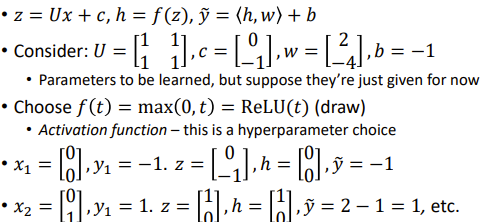
\includegraphics[width=9cm, height=3cm]{22.png}
    \end{minipage}
};
\node[fancytitle, right=10pt] at (box.north west) {[Multilevel Perceptron] 2 Layer Perceptron};
\end{tikzpicture}

\begin{tikzpicture}
\node [mybox] (box){%
    \begin{minipage}{0.44\textwidth}
	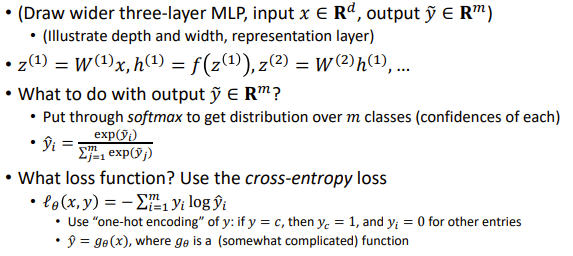
\includegraphics[width=9cm, height=4cm]{23.png}
    \end{minipage}
};
\node[fancytitle, right=10pt] at (box.north west) {[Multilevel Perceptron] 3 Layer Perceptron};
\end{tikzpicture}

\begin{tikzpicture}
\node [mybox] (box){%
    \begin{minipage}{0.44\textwidth}
	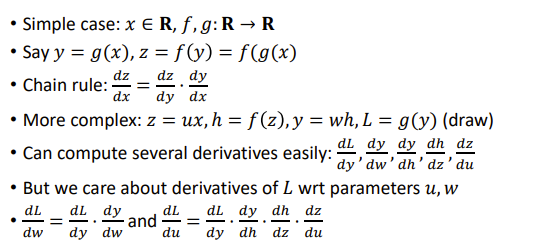
\includegraphics[width=9cm, height=3cm]{24.png}
    \end{minipage}
};
\node[fancytitle, right=10pt] at (box.north west) {[Multilevel Perceptron] Back Propagation};
\end{tikzpicture}

\begin{tikzpicture}
\node [mybox] (box){%
    \begin{minipage}{0.44\textwidth}
	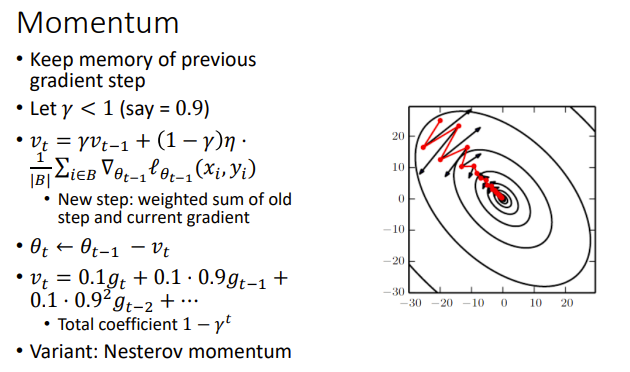
\includegraphics[width=9cm, height=3.5cm]{25.png}
    \end{minipage}
};
\node[fancytitle, right=10pt] at (box.north west) {[Deep Networks] Momentum };
\end{tikzpicture}

\begin{tikzpicture}
\node [mybox] (box){%
    \begin{minipage}{0.44\textwidth}
	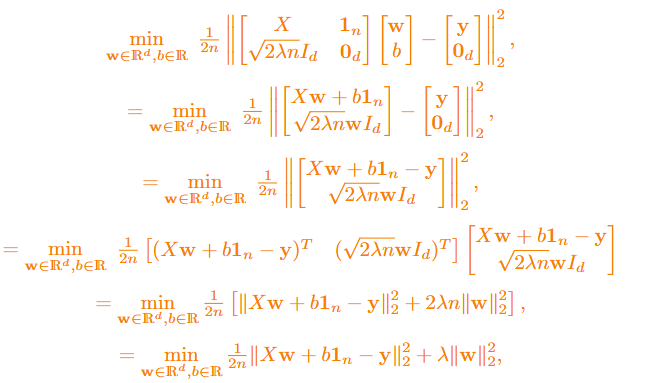
\includegraphics[width=9cm, height=5cm]{26.png}
    \end{minipage}
};
\node[fancytitle, right=10pt] at (box.north west) {[A \#1] Ridge Regression };
\end{tikzpicture}

\begin{tikzpicture}
\node [mybox] (box){%
    \begin{minipage}{0.44\textwidth}
	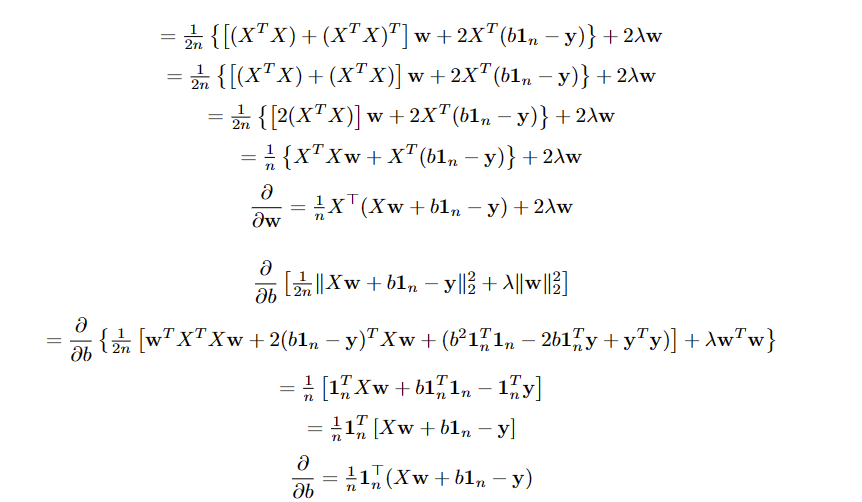
\includegraphics[width=9cm, height=5cm]{27.png}
    \end{minipage}
};
\node[fancytitle, right=10pt] at (box.north west) {[A \#1] Ridge Regression  Derivatives};
\end{tikzpicture}

\begin{tikzpicture}
\node [mybox] (box){%
    \begin{minipage}{0.44\textwidth}
	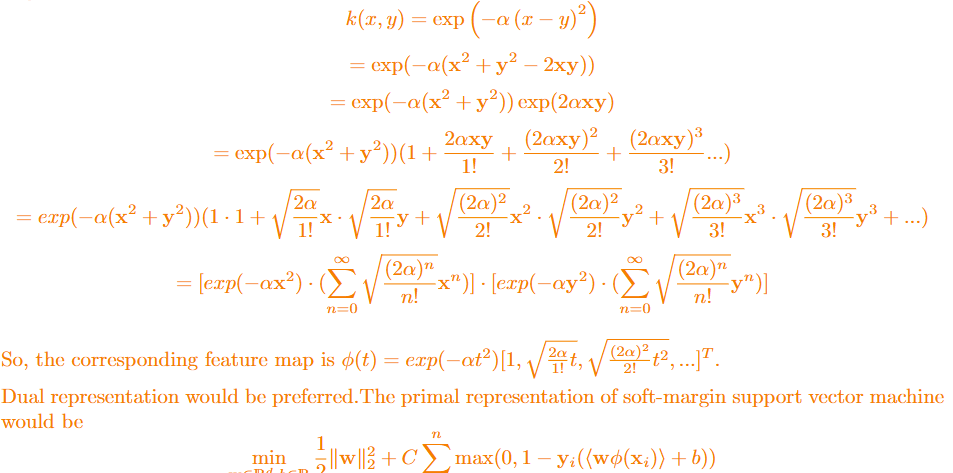
\includegraphics[width=9cm, height=5cm]{28.png}
    \end{minipage}
};
\node[fancytitle, right=10pt] at (box.north west) {[A \#2] Kernels};
\end{tikzpicture}

\begin{tikzpicture}
\node [mybox] (box){%
    \begin{minipage}{0.44\textwidth}
	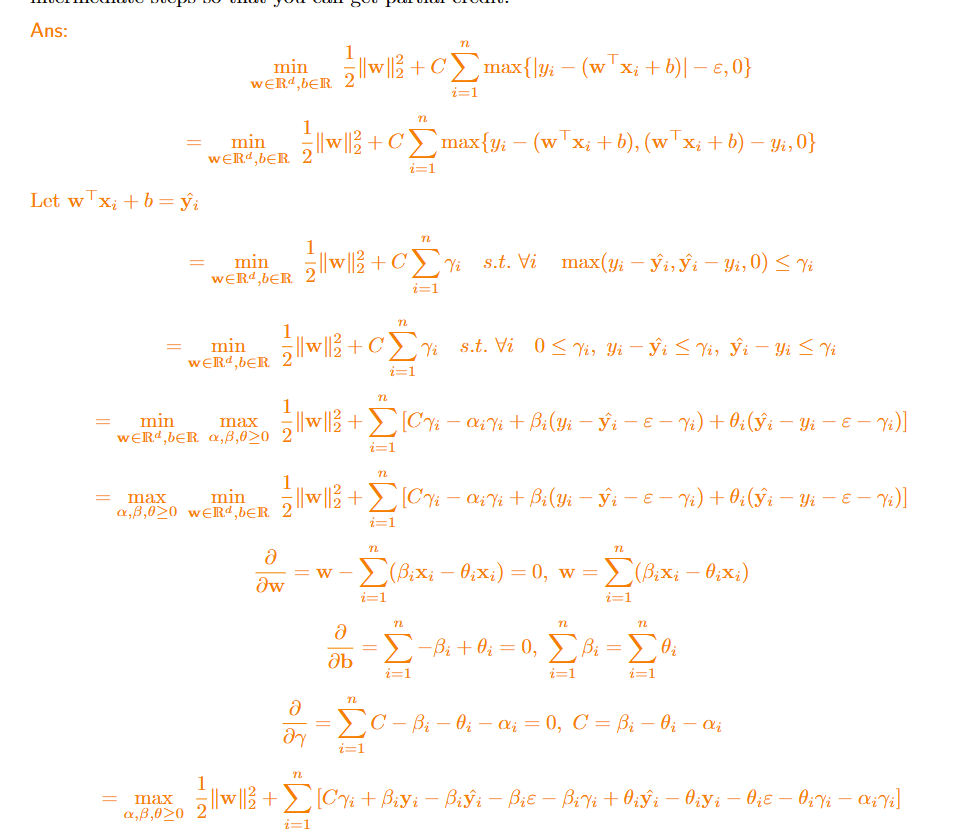
\includegraphics[width=9cm, height=8cm]{29.png}
    \end{minipage}
};
\node[fancytitle, right=10pt] at (box.north west) {[A \#2] Duels};
\end{tikzpicture}
\end{multicols*}
\end{center}
\end{document}